\newpage
\fancyhead[C]{Jihwan Shin}
\section{Mission Planning} \label{missionplanning}

\subsection{Objectives and Existing Works}

\iffalse
- list what the existing works on path planning use
- list what the existing companies for mine detection drones use as their algorithm if they can be found
\fi

The mission planning of the multi-aerial drone system focuses on how to efficiently plan the paths of the drones to survey our \gls{roi} using the chosen suite of sensors. The input will be the user-defined \gls{roi} and the specifications of the drone system, which goes through the mission planning algorithm to output the set of coordinates each drone must follow.

\begin{figure}
    \centering
    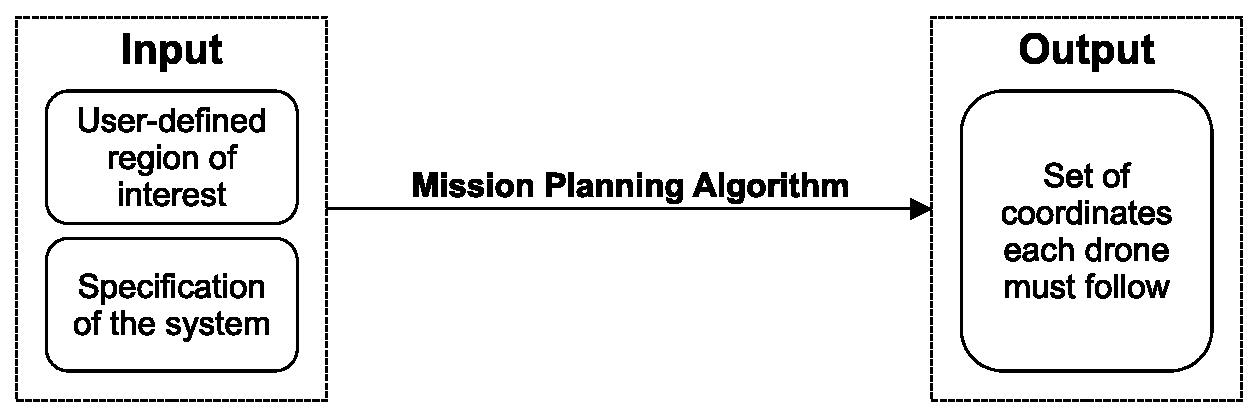
\includegraphics[width=0.5\linewidth]{figs/Objective of the Mission Planning System.eps}
    \caption{Objective of the Mission Planning System}
    \label{fig:objmsp}
\end{figure}

Existing works focus 

We aim to improve on these works by proposing a \textit{Layered Approach} to the mission planning of our drone system to optimise the time and resources required.  

\subsection{Layered Approach}

\iffalse
- mention the use of thermal and GPSAR sensors for detection
- explain what the layered approach is following the steps in the presentation
- form a mathematical equation for how much time it can save compared to previous methods
\fi

\begin{enumerate}
    \item \textbf{Define} the region of interest and obstacles.
    \item \textbf{Cover} the area using a thermal sensor through a \gls{cpp} algorithm.
    \item \textbf{Analyse} the thermal readings using a machine learning algorithm to find the suspected points.
    \item \textbf{Target} and rescan the suspected points using a \gls{gpr} sensor through a \gls{tspo} algorithm.
    \item \textbf{Confirm} the landmine locations with the \gls{gpr} readings. 
    \item \textbf{Demine} using the generated landmine location map. 
\end{enumerate}

\subsection{Defining the Region of Interest}

\iffalse
- explain Polygon with Holes data type in CGAL, and why it's an efficient why to describe our ROI
- explain the use of QGIS and how it's easy for an inexperienced operator to use
- explain the skeleton algorithm to give a border if required
- extension: using a deep-nn to automatically detect the likely locations?
\fi

\subsection{Coverage Path Planning}

\iffalse
- boustrophedon path planning. boustrophedon cell decomposition. previous research on this field.
- optimising with respect to the number of turns, distance, etc. 
- ASL cpp algorithm will be used on a virtual machine. explain how the algorithm works
\fi

\subsection{Travelling Salesman Problem with Obstacles}

\iffalse 
- what is a normal TSP
- how is TSP-O different from TSP
- how to simplify a TSP-O into a normal TSP by the use of visibility graph
- demonstration using a simple ROI (square within square) to show how it works
- time complexity and justification for our application (not real time, not too detailed roi)
\fi 

\subsection{Expanding to a Multi-Drone Operation}

\iffalse
- possible options such as straight line division but why i chose divide and cluster
- explanation of the divide and cluster algorithm
- delanauy triangulation, clustering algorithm
- time complexity (if it can be found) 
- appeal how expandable this would be for multi-aerial drone system 
\fi 

\subsection{Constraints}

\subsection{Real Location Example}

\subsection{Comparison with Manual Demining Operation}

\subsection{Future Work}